\section{Approach}

\subsection{B and B+ Backend}
    Our apporach to creating the backend which would handle the structure 
of the trees and their contents was fairly straight forward.  We had access to
well defined rules that define B and B+ trees so designing the general structure 
of the trees was simple enough.  However, since our intent was for the web interface 
to ba able to actively switch between B and B+ tree representations we had to factor 
in as much shared resources as we could to assist in the process of switching between 
the two tree types.  Conveniently, B and B+ trees are fairly similar, so it did not take
much extra effort to make much of the trees structure shared.  Specficially, both tree types
utilize the same node/block object we have created.  While the nodes have some properties 
unique to either type of tree, which comes at a slight memory cost, it makes it easier to 
switch back and forth.  We also keep a master list of all values in the tree at any given time.
This master list is the primary element that allows us to switch between tree structures.
Whenever we want to switch, we simply copy the element list, change the tree type, and then 
insert every value into the tree, in the same order they had been inserted into the previous 
tree.  It should be noted that this method could result in getting a different tree if you switched 
from B tree to B+ and back again, or vice versa.  this is because we do not execute all opperations 
that occurred on the previous tree, just insertions of values that were in it, so any imperfect 
organization caused by deletion could be cleaned up by switching back and orth between tree structures.
While structurally the trees have various commonalities, the methods of insertion, deletion, and searching 
the trees still had to remain completely separate due to the subtly differences in the tree structures.

The theory for the implementation was deceptively simple, since we had worked it out on paper in class, 
and the algorithms were simple enough to read through.  However general human intuition turned out to 
be fairly complicated to translate into usable Javascript code.  In order of complexity of implementation 
we had the general tree and node object structue, then the search methods, followed distantly by the insertion 
and deletion methods, which turned out to be quite complex to implement appropriately.
    Setting up the general structure for the objects that would represent our trees and the nodes that make them up 
was simple enough.  For B trees we created an object with properties to hold a master list of all nodes in the tree, 
the order of the tree, a direct reference to the tree's root node, a counter forthe number of nodes in the tree, and 
references to the methods for searching, insertion, and deletion methods, as well as a helper method called insertUp, 
which is called recursively after a node overflows to handle splitting the node and inserting the appropriate key into 
the parent node.  For B+ trees, the object we created has almost all the same properties, but it's insertUp method is 
only for internal node overflow handling, and it also has a reference to a methos called bp_leaf_split which handles 
overflow in a leaf node.  For nodes, we designed them to work with both tree types.  They contain a list of the values/keys 
in the node, a list of the children to the node, a reference to the node's parent, counters for the number of values/keys 
and for the number of children, a flag to signify if the node is a leaf node, and a reference to a helper method that returns 
the list of children to the node. The tree objects maintain a list of all the nodes in the tree because Javascript does not 
have easy to use pointers, so a master list had to be maintained so we could reference specific nodes as need be.  
As such, all references to nodes outside the master list, such as those inside nodes referencing children and its parent, are stored 
as the index of the node in the master list.  This method has the same memory footprint as a method that would have used pointers, 
though it adds a few extra lines of code where we have to constantly reference back to the trees node list and look up the index value 
of whatever node we want to reference.
    Implementing search for the two tree types was fairly straight forward and was accomplished in as few as 27 lines of code.  
For B trees, the method for searching consists of starting at the root, inspecting in the search value is in the node, if not 
then we decide which child node it would be in and then recursively call the search function starting from the child node the value 
should be in.  If we encounter a dead end and have not yet found our value, then we return that the value did not exist in the tree.
If we do find the value we return the index of the node it was found in and a true flag to indicate that the value was found.  The 
method for searching a B+ tree was similar except we do not check to see if the search value is in the current node until we've 
reached a leaf node.  Until we reach a leaf we just decide which child to explorenext and recursively call the search function 
starting from that child.  Once we've reached a leaf node, if we find the value in the node, we return the node index amd a true flag.
  If we reach a leaf node, and it does not contain our search value, then we return falseto indicate the value does not exist in the tree.

\begin{figure}[htp]
\centering
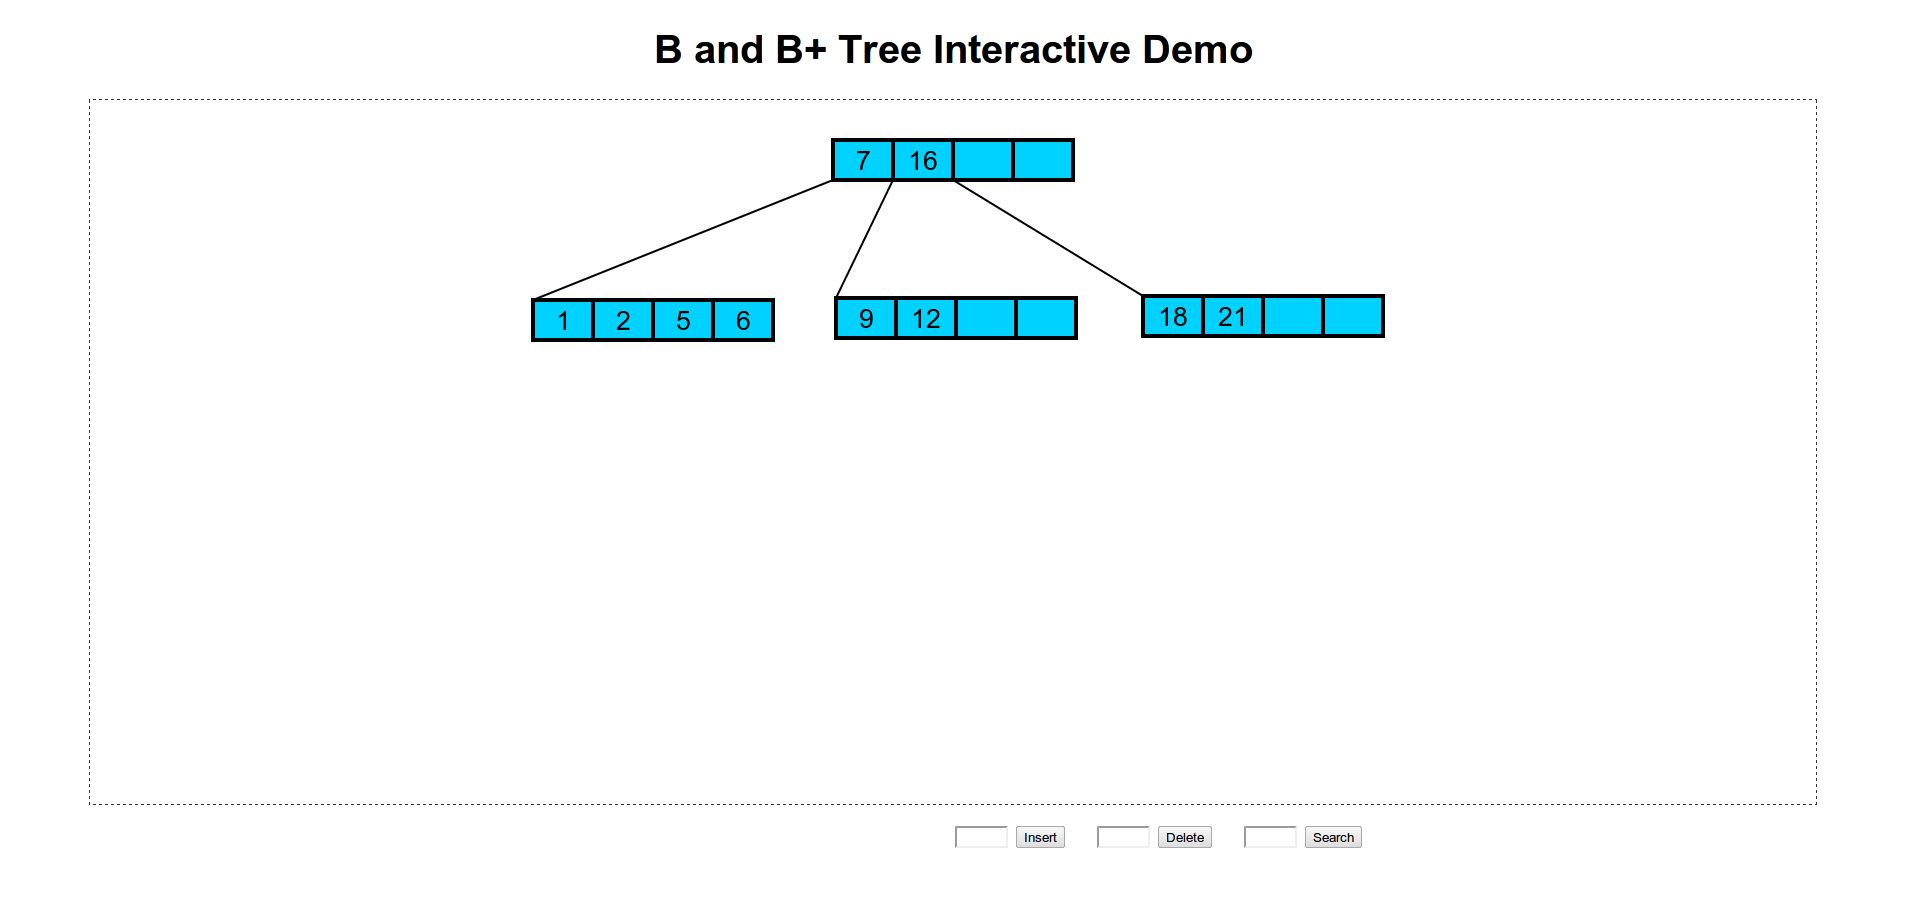
\includegraphics[scale=0.25]{images/Interface.png}
\caption{The user interface of our project}
\label{UI}
\end{figure}
